% ****** Start of file apssamp.tex ******
%
%   This file is part of the APS files in the REVTeX 4.1 distribution.
%   Version 4.1r of REVTeX, August 2010
%
%   Copyright (c) 2009, 2010 The American Physical Society.
%
%   See the REVTeX 4 README file for restrictions and more information.
%
% TeX'ing this file requires that you have AMS-LaTeX 2.0 installed
% as well as the rest of the prerequisites for REVTeX 4.1
%
% See the REVTeX 4 README file
% It also requires running BibTeX. The commands are as follows:
%
%  1)  latex apssamp.tex
%  2)  bibtex apssamp
%  3)  latex apssamp.tex
%  4)  latex apssamp.tex
%
\documentclass[%
 reprint,
%superscriptaddress,
%groupedaddress,
%unsortedaddress,
%runinaddress,
%frontmatterverbose, 
%preprint,
%showpacs,preprintnumbers,
nofootinbib,
%nobibnotes,
%bibnotes,
 amsmath,amssymb,
 aps,
%pra,
%prb,
%rmp,
%prstab,
%prstper,
%floatfix,
]{revtex4-1}

\usepackage{graphicx}% Include figure files
\usepackage{dcolumn}% Align table columns on decimal point
\usepackage{bm}% bold math
\usepackage{amssymb}
\usepackage{amsmath}
\usepackage{graphicx}
\usepackage{courier}


\DeclareMathOperator*{\argmax}{arg\,max}
\DeclareMathOperator*{\argmin}{arg\,min}

\newcommand{\abs}[1]{\left\|{#1}\right\|}

%\usepackage{hyperref}% add hypertext capabilities
%\usepackage[mathlines]{lineno}% Enable numbering of text and display math
%\linenumbers\relax % Commence numbering lines

%\usepackage[showframe,%Uncomment any one of the following lines to test 
%%scale=0.7, marginratio={1:1, 2:3}, ignoreall,% default settings
%%text={7in,10in},centering,
%%margin=1.5in,
%%total={6.5in,8.75in}, top=1.2in, left=0.9in, includefoot,
%%height=10in,a5paper,hmargin={3cm,0.8in},
%]{geometry}

\begin{document}

%\preprint{APS/123-QED}

\title{Regional Trends in Misrepresenting MDMA}% Force line breaks with \\
%\thanks{A footnote to the article title}%

\author{Burke Brockelbank}

\date{\today}% It is always \today, today,
             %  but any date may be explicitly specified

\begin{abstract}

\end{abstract}

\maketitle

%\tableofcontents
\section{\label{sec:Introduction}Introduction}
EcstasyData.org is an independent laboratory pill testing program run by Erowid Center with support from Isomer Design and Dancesafe. Its purpose is to collect, review, manage, and publish laboratory testing results from our lab and republished from other analysis projects worldwide.

\begin{figure*}
  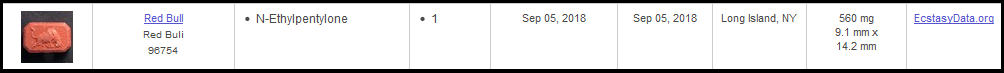
\includegraphics[width=0.9\textwidth]{example.png}
  \caption{An example of testing data obtained by EcstasyData.org. } \label{fig:DataExample}
\end{figure*}

The database consists of sets of data exemplified by Figure \ref{fig:DataExample}. Pills are supplied by people all over the world to be tested for composition. The origin city as well as the what the pill was sold as are recorded.

We want to use a self-organizing map on the data to find regional trends.

\section{\label{sec:Methods}Methods}

	Locations are stored as cities, but we want to look at their locations on the globe. First we simply need to get the lattitude and longitude of a given city which we do with geopy. Then we need to turn this into a form where nearby locations have similar coordinates. This becomes an issue because longitude is modular. A solution to this is to make a change of coordinates into cartesian coordinates.

	\begin{equation}
		(x, y, z) = R \left(\cos(\text{lon})\cos(\text{lat}), \sin(\text{lon})\cos(\text{lat}), \sin(\text{lat})\right) \eqref{eq:coordinate}
	\end{equation}

	Although the difference between two cartesian coordinates does not represent the distance over land between two points, it makes no distance to clustering because for any three cartesian coordinates $A$, $B$, and $C$, if $A$ and $B$ are closer than $A$ and $C$, then

	\begin{equation}
		\abs{A-B} < \abs{A-C}.
	\end{equation}

	This means that clusters of points in the cartesian coordinate attributes accurately reflects clustering due to proximity.

We will probably have better luck classifying chemicals as

Ecstasy-like Chemicals : MDA, MDE, 4-FA, Methylone, 4-Methylmethcathinone
Psychedelics : 2C-B, 5-MeO-DiPT, DOB, PMA, 5-MeO-DALT, 5-MeO-DPT, Bromo-dragonfly, 2C-I, AL-LAD, 25B-NBOMe, 25C-NBOMe, 25I-NBOMe
Cannabinoids : AB-PINACA, JWH-018, JWH-073, JWH-081, JWH-210, JWH-250, JWH-359, AB-CHMINACA, AB-FUBINACA, THC, Thermoliz UR-144F, UR-144, 5-fluoro-AMB, 5-fluoro-ADB , ADB-CHMINACA, ADB-FUBINACA, AMB-FUBINACA, NM-2201, U-47700, XLR-11
Dissociatives : DXM, Ketamine, PCP
Stimulants : Amphetamines, BZP, Caffeine, Cocaine, Methamphetamine, Pseudo/Ephedrine, TFMPP, MDPV, Dimethylcathinone, MDAI, Ethylamphetamine, Dibenzylpiperazine, mCPP, Modafinil, Phentermine
Depressants/Tranquilizers : Amitriptyline, Butabarbital, Carisoprodol, Codeine, Diazepam, Diphenhydramine, Oxycodone, Lorazepam, Dihydrocodeine, Fentanyl, Phenobarbital
Non-Psychoactive Substances : Acetaminophen, Aspirin, Chlorpheniramine, Guaifenesin, Methyl Salicylate, Methandrostenolone, Phenylpropanolamine, Niacinamide, Ibuprofen, Procaine

I need to find out how to deal with the interchangability of chemicals in the mix. I.e. if a pill is half MDMA half MDA, it should get classified the same as a pill which is half MDA and half MDMA. If I categorize the chemicals by type, I can just have each type be an attribute and then the value for the data point is its percentage

\section{\label{sec:Results}Results}


\section{\label{sec:Discussion}Discussion}


%\bibliographystyle{apsrev4-1}
%\bibliography{bib}

\end{document}

%
% ****** End of file apssamp.tex ******



























